% !TEX root=../root.tex

\subsection{Feature Tracking}
As mentioned in~\secref{sec:estimation},
the estimation algorithm uses measurements of visual features that are
rigidly attached to the landing target vehicle. It is important to note that
determining which visual features in a camera image are attached to
the target vehicle is not a trivial problem. We leave this problem as future work and
circumvent this problem by flying low enough to the target vehicle such that it
occupies the entire field of view of the camera.

Visual features were first detected using a FAST feature
detector~\cite{rosten2006machine}. The detected features were then tracked from one frame to
the next using optical flow~\cite{bouguet2001pyramidal}.
To remove features that had been poorly tracked, we periodically
estimated the essential matrix between the current camera image
and a stored keyframe.
Outliers to this estimated essential matrix were discarded, and new FAST
features were detected to replace them.
% to have been poorly tracked
% Periodically, we
% removed
% features that had been poorly tracked by estimating the essential matrix between
% the current camera image and a stored keyframe image. Outliers to the found
% essential matrix were thrown out, and new FAST features were detected to replace
% them. 
For our experiments, the feature tracker attempted to maintain 250
tracked features at all times. As the proposed estimator only used ten visual
features at a time,
% measurements from a few
% tracked features,
a subset of the tracked features which had persisted the longest
were provided to the estimator for each camera image.

Each visual feature that was acquired and tracked was assigned a unique integer
identitication number. The estimator used these identification numbers to
determine when visual features were no longer tracked and when new visual
features were acquired.
% a visual feature was no longer tracked and, therefore, should
% have been removed from
% the estimated state.
An example camera image from the UAV showing the
subset of tracked features provided to the estimator with the corresponding
identification
numbers is seen in~\figref{fig:features_with_aruco}.


\begin{figure}
  \centering
  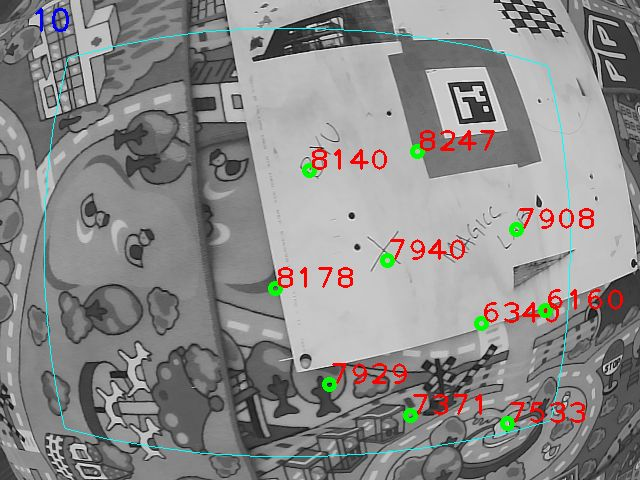
\includegraphics[scale=0.5]{imgs/features_with_aruco.png}
  \caption[Visual Feature Tracking During Flight Experiment]{A processed camera image from the multirotor UAV's camera. The ArUco
  marker is pictured in the top, right corner of the image. Each green
circle shows the tracked location of a visual feature used by the
estimator. The red number associated with each visual feature is the unique
integer ID assigned by the feature tracker.}
  \label{fig:features_with_aruco}
\end{figure}
